\chapter{Organización Empresarial}
La estructura organizativa planteada para el proyecto de investigación está basada de forma ideal en el \textit{Área de Investigación de análisis de datos} de un \textit{Instituto de Cancerología}. 

\section{Misión}
Somos una institución que trabaja por el control integral del cáncer a través de la atención y el cuidado de pacientes, la investigación, la formación de talento humano y el desarrollo de acciones en salud pública.

\section{Visión}
En 2026 el Instituto de Cancerología será referente por sus logros en la reducción de la mortalidad por cáncer, sobre la base de la innovación y la tecnología, con un actuar ético y sostenible y con un talento humano motivado y
comprometido.
\newpage

\section{Objetivo}
La investigación en su formulación y desarrollo genera dudas o problemas de carácter estadístico que necesitan un enfoque experto. El  Área de Investigación de Análisis de datos tiene por objetivo dar soporte a los investigadores de la Subdirección de Investigaciones, otras Subdirecciones y demás unidades funcionales del Instituto de Cancerología, en métodos para el manejo y análisis de datos, a través de las siguientes actividades:

\begin{itemize}
\item Proponer e implementar estrategias que permitan mantener una calidad elevada en el análisis de datos de los proyectos de investigación de la Subdirección de Investigaciones, otras Subdirecciones y demás unidades funcionales del Instituto de Cancerología.
\item Apoyar el diseño de base de datos y el desarrollo de soluciones informáticas para la captura de información de  los proyectos de investigación  y otros proyectos del Instituto de Cancerología.
\item Administrar las bases de datos de los proyectos de investigación desarrollados por el Instituto de Cancerología.
\item Desarrollar soluciones informáticas que permitan la sistematización de los diferentes procesos relacionados con la gestión y análisis de datos resultado de proyectos de investigación u otros proyectos del Instituto de Cancerología.
\item Apoyar, desde el punto de vista estadístico, la formulación de proyectos de investigación.
\item Elaborar e implementar el plan de análisis estadístico de los proyectos de investigación.
\item Apoyar los procesos de publicación científica en el componente de análisis de datos.
\item Proponer e implementar mecanismos que permitan hacer seguimiento a la ejecución de proyectos de investigación.
\item Desarrollar  modelos de simulación para estudios de evaluación económica.
\item Desarrollar modelos de simulación para la toma de decisiones en salud.
\end{itemize}

\newpage
\section{Actores,Roles y Funciones}
Los actores, Roles y funciones que conforman La jerarquía del \textit{Área de Investigación de análisis de datos} puede ser observada en la Figura\ref{organigrama}

\begin{center}
\begin{figure}[h!]
	\centering
	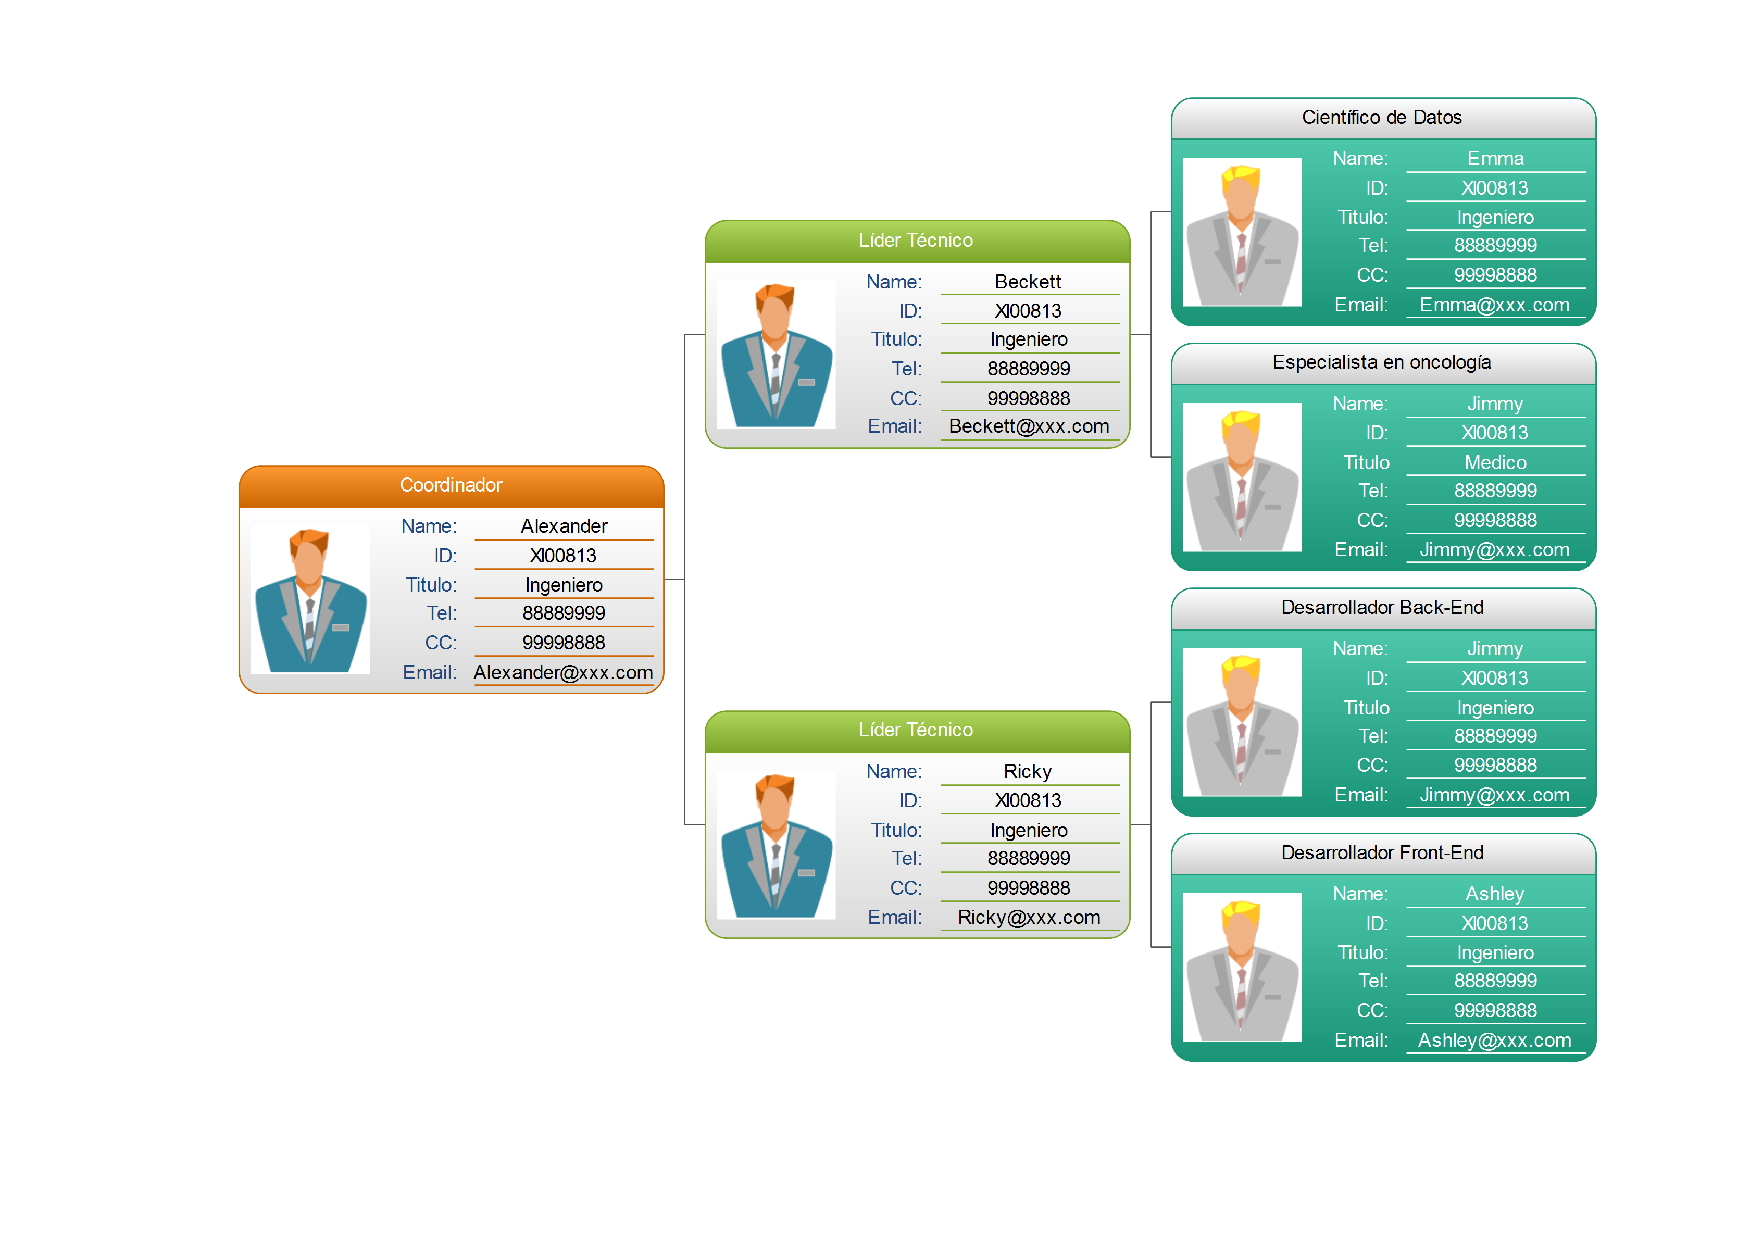
\includegraphics[width=1\linewidth]{ARQUITECTURA/imgs/organizacion}
	\caption{Jerarquía del  Área de Investigación de análisis de datos}
	\label{organigrama}
\end{figure}
\end{center}
\newpage
\section{Servicios}
El grupo de análisis de datos ofrece los siguientes servicios:
\begin{itemize}
	\item Desarrollo de modelos de decisión (árboles de decisión, modelos de Markov, simulación de eventos discretos y simulación dinámica).
	\item Desarrollo de modelos estadísticos predictivos y explicativos.
	\item Análisis de datos avanzados (modelos lineales generalizados, análisis multinivel, etc.).
	\item Análisis bioinformáticas.
	\item Estadística espacial.
	\item Minería de datos.
	\item Diseños de formularios para la captura electrónica de información (web, escritorio, apps, etc.).
	\item Administración de bases de datos.
	\item Elaboración de proyectos de investigación (métodos).
	\item Programación en R, SAS, SPSS, Stata.
	\item Evaluación económica
\end{itemize}


